\documentclass{standalone}
\usepackage{tikz}
\usepackage{ctex,siunitx}
\setCJKmainfont{Noto Serif CJK SC}
\usepackage{tkz-euclide}
\usepackage{amsmath}
\usepackage{wasysym}
\usetikzlibrary{patterns, calc}
\usetikzlibrary {decorations.pathmorphing, decorations.pathreplacing, decorations.shapes,}
\begin{document}
\small
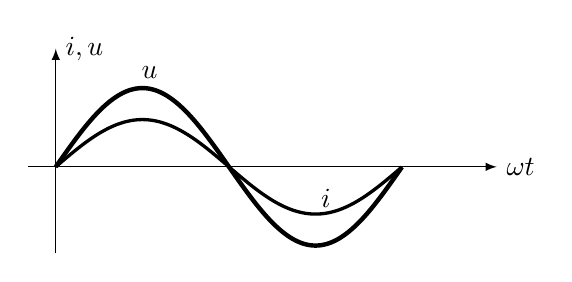
\begin{tikzpicture}[>=latex,xscale=0.7]
  % \useasboundingbox(0.9,0)rectangle(5.1,5);
  \draw [->](-.5,0)--(8,0)node[right]{$\omega t$};
  \draw [->](0,-1.1)--(0,1.5)node[right]{$i, u$};
  \draw [ultra thick,domain=0:2*pi, samples=1000] plot (\x,{sin(\x r)});
  \draw [very thick,domain=0:2*pi, samples=1000] plot (\x,{0.6*sin(\x r)});
\node at (1.7,1.2){$u$};
\node at (4.9,-.4){$i$};
\end{tikzpicture}
\end{document}